\documentclass[a4paper, 12pt]{article}%тип документа

%отступы
\usepackage[left=2cm,right=2cm,top=2cm,bottom=3cm,bindingoffset=0cm]{geometry}

%Русский язык
\usepackage[T2A]{fontenc} %кодировка
\usepackage[utf8]{inputenc} %кодировка исходного кода
\usepackage[english,russian]{babel} %локализация и переносы

%Вставка картинок
\usepackage{wrapfig}
\usepackage{graphicx}
\graphicspath{{pictures/}}
\DeclareGraphicsExtensions{.pdf,.png,.jpg}

%оглавление
\usepackage{titlesec}
\titlespacing{\chapter}{0pt}{-30pt}{12pt}
\titlespacing{\section}{\parindent}{5mm}{5mm}
\titlespacing{\subsection}{\parindent}{5mm}{5mm}
\usepackage{setspace}

%Графики
\usepackage{multirow}
\usepackage{pgfplots}
\pgfplotsset{compat=1.9}

%Математика
\usepackage{amsmath, amsfonts, amssymb, amsthm, mathtools}

%Заголовок
\author{Валеев Рауф Раушанович \\
группа 825}
\title{\textbf{Работа 2.1.1\\
Измерение магнитного поля Земли}}
\newtheorem{task}{Задача}
\begin{document}
\maketitle
\newpage
\section*{Цель работы}
Определить характеристики шарообразных неодимовых магнитов и, используя законы взаимодействия магнитных моментов с полем, измерить горизонтальную и вертикальную составляющие индукции магнитного поля Земли и магнитное наклонение.
\section*{В работе используются}
12 одинаковых неодимовых магнитных шариков, тонкая нить для изготовления крутильного маятника, медная проволока диаметром ($0,5 - 0,6$) мм, электронные весы, секундомер, измеритель магнитной индукции АТЕ-8702, штангенциркуль, брусок из немагнитного материала ($25\times30\times60$ мм$^3$), деревянная линейка, штатив из немагнитного материала; дополнительные неодимовые магнитные шарики ($\sim$ 20 шт.) набор гирь и разновесов.
\section*{Теоретическая справка}
\subsection*{Точечный магнитный диполь}
Простейший магнитный диполь может быть образован витком с током или постоянным магнитом. По определению, магнитный момент $\vec{P_m}$ тонкого витка площадью $S$ с током $I$ равен:
\begin{equation*}
\vec{P_m} = \dfrac{I}{c}\vec{S} = \dfrac{I}{c} S \vec{n}
\end{equation*} 
где $c$ – скорость света в вакууме, $\vec{S} = S \vec{n}$ — вектор площади контура, образующий с направлением тока правовинтовую систему, $\vec{n}$ --- единичный вектор нормали к площадке $S$ (это же направление $\vec{P}_m$ принимается за направление $S \to N$ от южного ($S$) к северному ($N$) полюсу). Если размеры контура с током или магнитной стрелки малы по сравнению расстоянием до диполя, то соответствующий магнитный диполь $\vec{P}_m$ называют элементарным или точечным.

Поле точечного диполя определяется по следующей формуле:
\begin{equation*}
\vec{B} = \dfrac{3\left(\vec{P_m}, \vec{r}\right)\vec{r}}{r^5} - \dfrac{\vec{P}_m}{r^3}
\end{equation*}
В магнитном поле с индукцией $\vec{B}$ на точечный магнитный диполь $\vec{P}_m$ действует механический момент сил:
\begin{equation*}
\vec{M} = \left[\vec{P_m}, \vec{B}\right]
\end{equation*}
Под действием вращающего момента $\vec{M}$ виток с током или постоянный магнит поворачивается так, чтобы его магнитный момент выстроился вдоль вектора индукции магнитного поля. Это --- положение устойчивого равновесия: при отклонении от этого положения возникает механический момент внешних сил, возвращающий диполь к положению равновесия. В положении, когда $\vec{P_m}$ и $\vec{B}$ параллельны, но направлены противоположно друг другу, также имеет место равновесие ($M = 0$), но такое равновесие неустойчиво: малейшее отклонение от этого положения приведёт к появлению момента сил, стремящихся отклонить диполь ещё дальше от начального положения.

Магнитный диполь в магнитном поле обладает энергией:
\begin{equation*}
W = -\left(\vec{P_m}, \vec{B}\right)
\end{equation*}
\subsection*{Неодимовые магниты}
В настоящей работе используются неодимовые магниты шарообразной формы.
Для нас важно то, что:
\begin{enumerate}
\item шары намагничены однородно;
\item вещество, из которого изготовлены магниты, является магнитожёстким материалом.
\end{enumerate}
Внутри такого шара магнитное поле равно 
\begin{equation}
B_0 = \dfrac{2P_m}{R^3}
\end{equation}
Полный магнитный момент $\vec{P_m}$ постоянного магнита определяется намагниченностью $\vec{p_m}$ вещества, из которого он изготовлен. По определению, намагниченность --- это магнитный момент единицы объёма. Для однородно намагниченного шара намагниченность, очевидно, равна:
\begin{equation}
\vec{p_m} = \dfrac{\vec{P_m}}{V}
\end{equation}
Намагниченность — важная характеристика вещества постоянных магнитов, определяющая, в частности, величину остаточной магнитной индукции $B_r = 4 \pi p_m$ (остаточная индукция $B_r$ --- одна из величин, которая, как правило, указывается в справочниках по магнитожёстким материалам).
\begin{equation}
\vec{B_P} = \dfrac{8\pi}{3}\vec{p_m} = \dfrac{2}{3} \vec{B_r}
\end{equation}
\subsection*{Экспериментальное определение величины магнитного момента магнитных шариков}
$P_m$ можно определить из параметров шарика и из расстояния $r_{max}$, на котором они удерживаются в поле тяжести.
\begin{equation}
P_m = \sqrt{\dfrac{mgr_{max}^4}{6}}
\end{equation}
\begin{equation}
\vec{B_p} = \dfrac{2\vec{P_m}}{R^3}
\end{equation}
\subsection*{Определение величины магнитного момента по силе сцепления магнитных шариков}
Если сила сцепления двух одинаковых шаров равна 
\begin{equation}
F_0 = \dfrac{6P_m^2}{d^4} \Rightarrow P_m = \sqrt{\dfrac{F_0d^4}{6}}
\end{equation}
то минимальный вес цепочки, при которой она оторвется от верхнего шарика равен:
\begin{equation}
F \approx 1,08F_0
\end{equation}
\subsection*{Измерение горизонтальной составляющей индукции магнитного поля Земли}
\begin{wrapfigure}{r}{0.25\textwidth}
  \begin{center}
    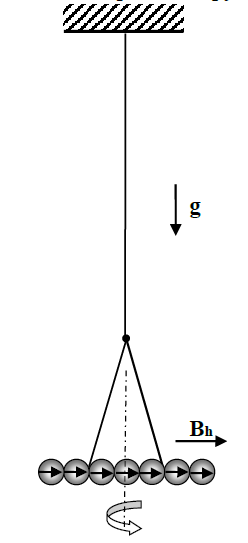
\includegraphics[width = 0.25\textwidth]{1.png}
  \end{center}
  \textbf{\caption{Крутильный маятник}}
\end{wrapfigure}
При отклонении "стрелки" на угол $\theta$ от равновесного положения в горизонтальной плоскости возникают крутильные колебания вокруг вертикальной оси, проходящей через середину стрелки. Если пренебречь упругостью нити, то уравнение крутильных колебаний такого маятника определяется возвращающим моментом сил $M = -P_0B_h \sin \theta$, действующим на "стрелку" со стороны магнитного поля Земли, и моментом инерции $I_n$ "стрелки" относительно оси вращения.\\
При малых амплитудах:
\[T = 2\pi \sqrt{\dfrac{I_n}{nP_mB_h}}\]
Пусть 
\[T(n) = kn \Rightarrow\]
\begin{equation}
k = \pi \sqrt{\dfrac{md^2}{3P_m B_h}} \Rightarrow B_h = \dfrac{\pi^2md^2}{3k^2P_m}
\end{equation}
\subsection*{Измерение вертикальной составляющей индукции магнитного поля Земли. Магнитное наклонение.}
С помощью небольшого дополнительного грузика "стрелку" можно "выровнять", расположив её горизонтально: в этом случае момент силы тяжести груза относительно точки подвеса будет равен моменту сил, действующих на "стрелку" со стороны магнитного поля Земли. Если масса уравновешивающего груза равна $m$, плечо силы тяжести $r$, а полный магнитный момент "стрелки" $P_0 = nP_m$, то в равновесии:
\[mgr = P_0 B_v = nP_mB_v\]
Пусть $M(n) = An \Rightarrow$
\begin{equation}
B_v = \dfrac{A}{P_m}
\end{equation}
\section*{Ход работы}
\subsection*{Определение магнитного момента, намагниченности и остаточной магнитной индукции вещества магнитных шариков}
\subsubsection*{Метод A}
Определим все данные наших шариков и запишем их в таблицу.\\
\begin{center}
\begin{tabular}{|c|c|c|}
\hline
Параметр & Значение & $\sigma$ \\ \hline
$m$, г & 0,85 & 0,01 \\ \hline
$d$, мм & 6 & 0,1 \\ \hline
\end{tabular}\\
\textbf{Таблица 1.} Параметры шариков.
\end{center}
Определим $r_{max}$. Затем по формуле $(3)$ определим $P_m$, по формуле $(2)$ определим $p_m$, по формуле $(5)$ определим $B_p$ и по формуле $(3)$ определим $B_r$. Все полученные данные занесем в таблицу 2
\begin{center}
\begin{tabular}{|c|c|c|}
\hline
Величина & Значение & $\sigma$ \\ \hline
$r_{max}$, см & 2,38 & 0,01 \\ \hline
$P_m$, Гс $\cdot$ см$^3$ & 67 & 2 \\ \hline
$p_m$, Гс & 590 & 30 \\ \hline
$B_p$, кГс & 4,9 & 0,2 \\ \hline
$B_r$, кГс & 7,4 & 0,3 \\ \hline
\end{tabular}\\
\textbf{Таблица 2.} Величины, определяемые в методе А.
\end{center}
Меряем $B_p$ с помощью магнитометра и получаем $B_p = (340 \pm 1)$ мТл.
\subsubsection*{Метод B}
Составим цепочку и определим $F$ - вес грузиков, которые надо подвесить к этой цепочке, чтобы грузики оторвались. 

По формуле $(7)$ определим силу сцепления двух шаров. По формуле $(6)$ найдем $P_m$ и запишем все данные в таблицу.
\begin{center}
\begin{tabular}{|c|c|c|}
\hline
Величина & Значение & $\sigma$ \\ \hline
$M$, г & 383,4 & 0,1 \\ \hline
$F$, кдин & 375,7 & 0,1 \\ \hline
$F_0$, кдин & 347,9 & 0,1 \\ \hline
$P_m$, Гс $\cdot$ см$^3$ & 86 & 3 \\ \hline
\end{tabular}\\
\textbf{Таблица 3.} Величины, определяемые в методе B.
\end{center}
В итоге получаем, что $P_m = (86 \pm 3)$ Гс $\cdot$ см$^3$. $B_p = (650 \pm 30)$ мТл, а $B_r = (960 \pm 40)$ мТл, что очень близко к табличным значениям ($1,03 - 1,13$ Тл), но довольно далеко от измеренного нами поля магнитометром.
\subsection*{Определение горизонтальной составляющей магнитного поля Земли}
Для определения горизонтальной составляющей магнитного поля Земли нам нужно собрать установку для возбуждения крутильных колебаний и исследовать зависимость количество шариков от периода. 

Перед этим удостоверимся, что при расчете периода упругость нити можно не учитывать, свернув стрелку в кольцо и измерив период крутильных колебаний (очевидно, что магнитный момент такой стрелки равен 0). Получаем $T = 50$ с. Это означает, что мы можем пренебречь упругостью нитей.
\begin{center}
\begin{tabular}{|c|c|c|c|}
\hline
$n$ & $t$, с & $N$ & $T$, с \\ \hline
12 & 34 & 10 & 3,4 \\ \hline
11 & 31 & 10 & 3,1 \\ \hline
10 & 28 & 10 & 2,8 \\ \hline
9 & 27,5 & 10 & 2,75 \\ \hline
8 & 22,5 & 10 & 2,25 \\ \hline
7 & 19,5 & 10 & 1,95 \\ \hline
6 & 16,5 & 10 & 1,65 \\ \hline
5 & 14,5 & 10 & 1,45 \\ \hline
4 & 11,5 & 10 & 1,15 \\ \hline
\end{tabular}\\
\textbf{Таблица 4. } Зависимость крутильных колебаний от количества шариков $T(n)$
\end{center}
Построим график зависимости $T(n)$ и по формуле $(8)$ найдем $B_h$.\\
\begin{center}
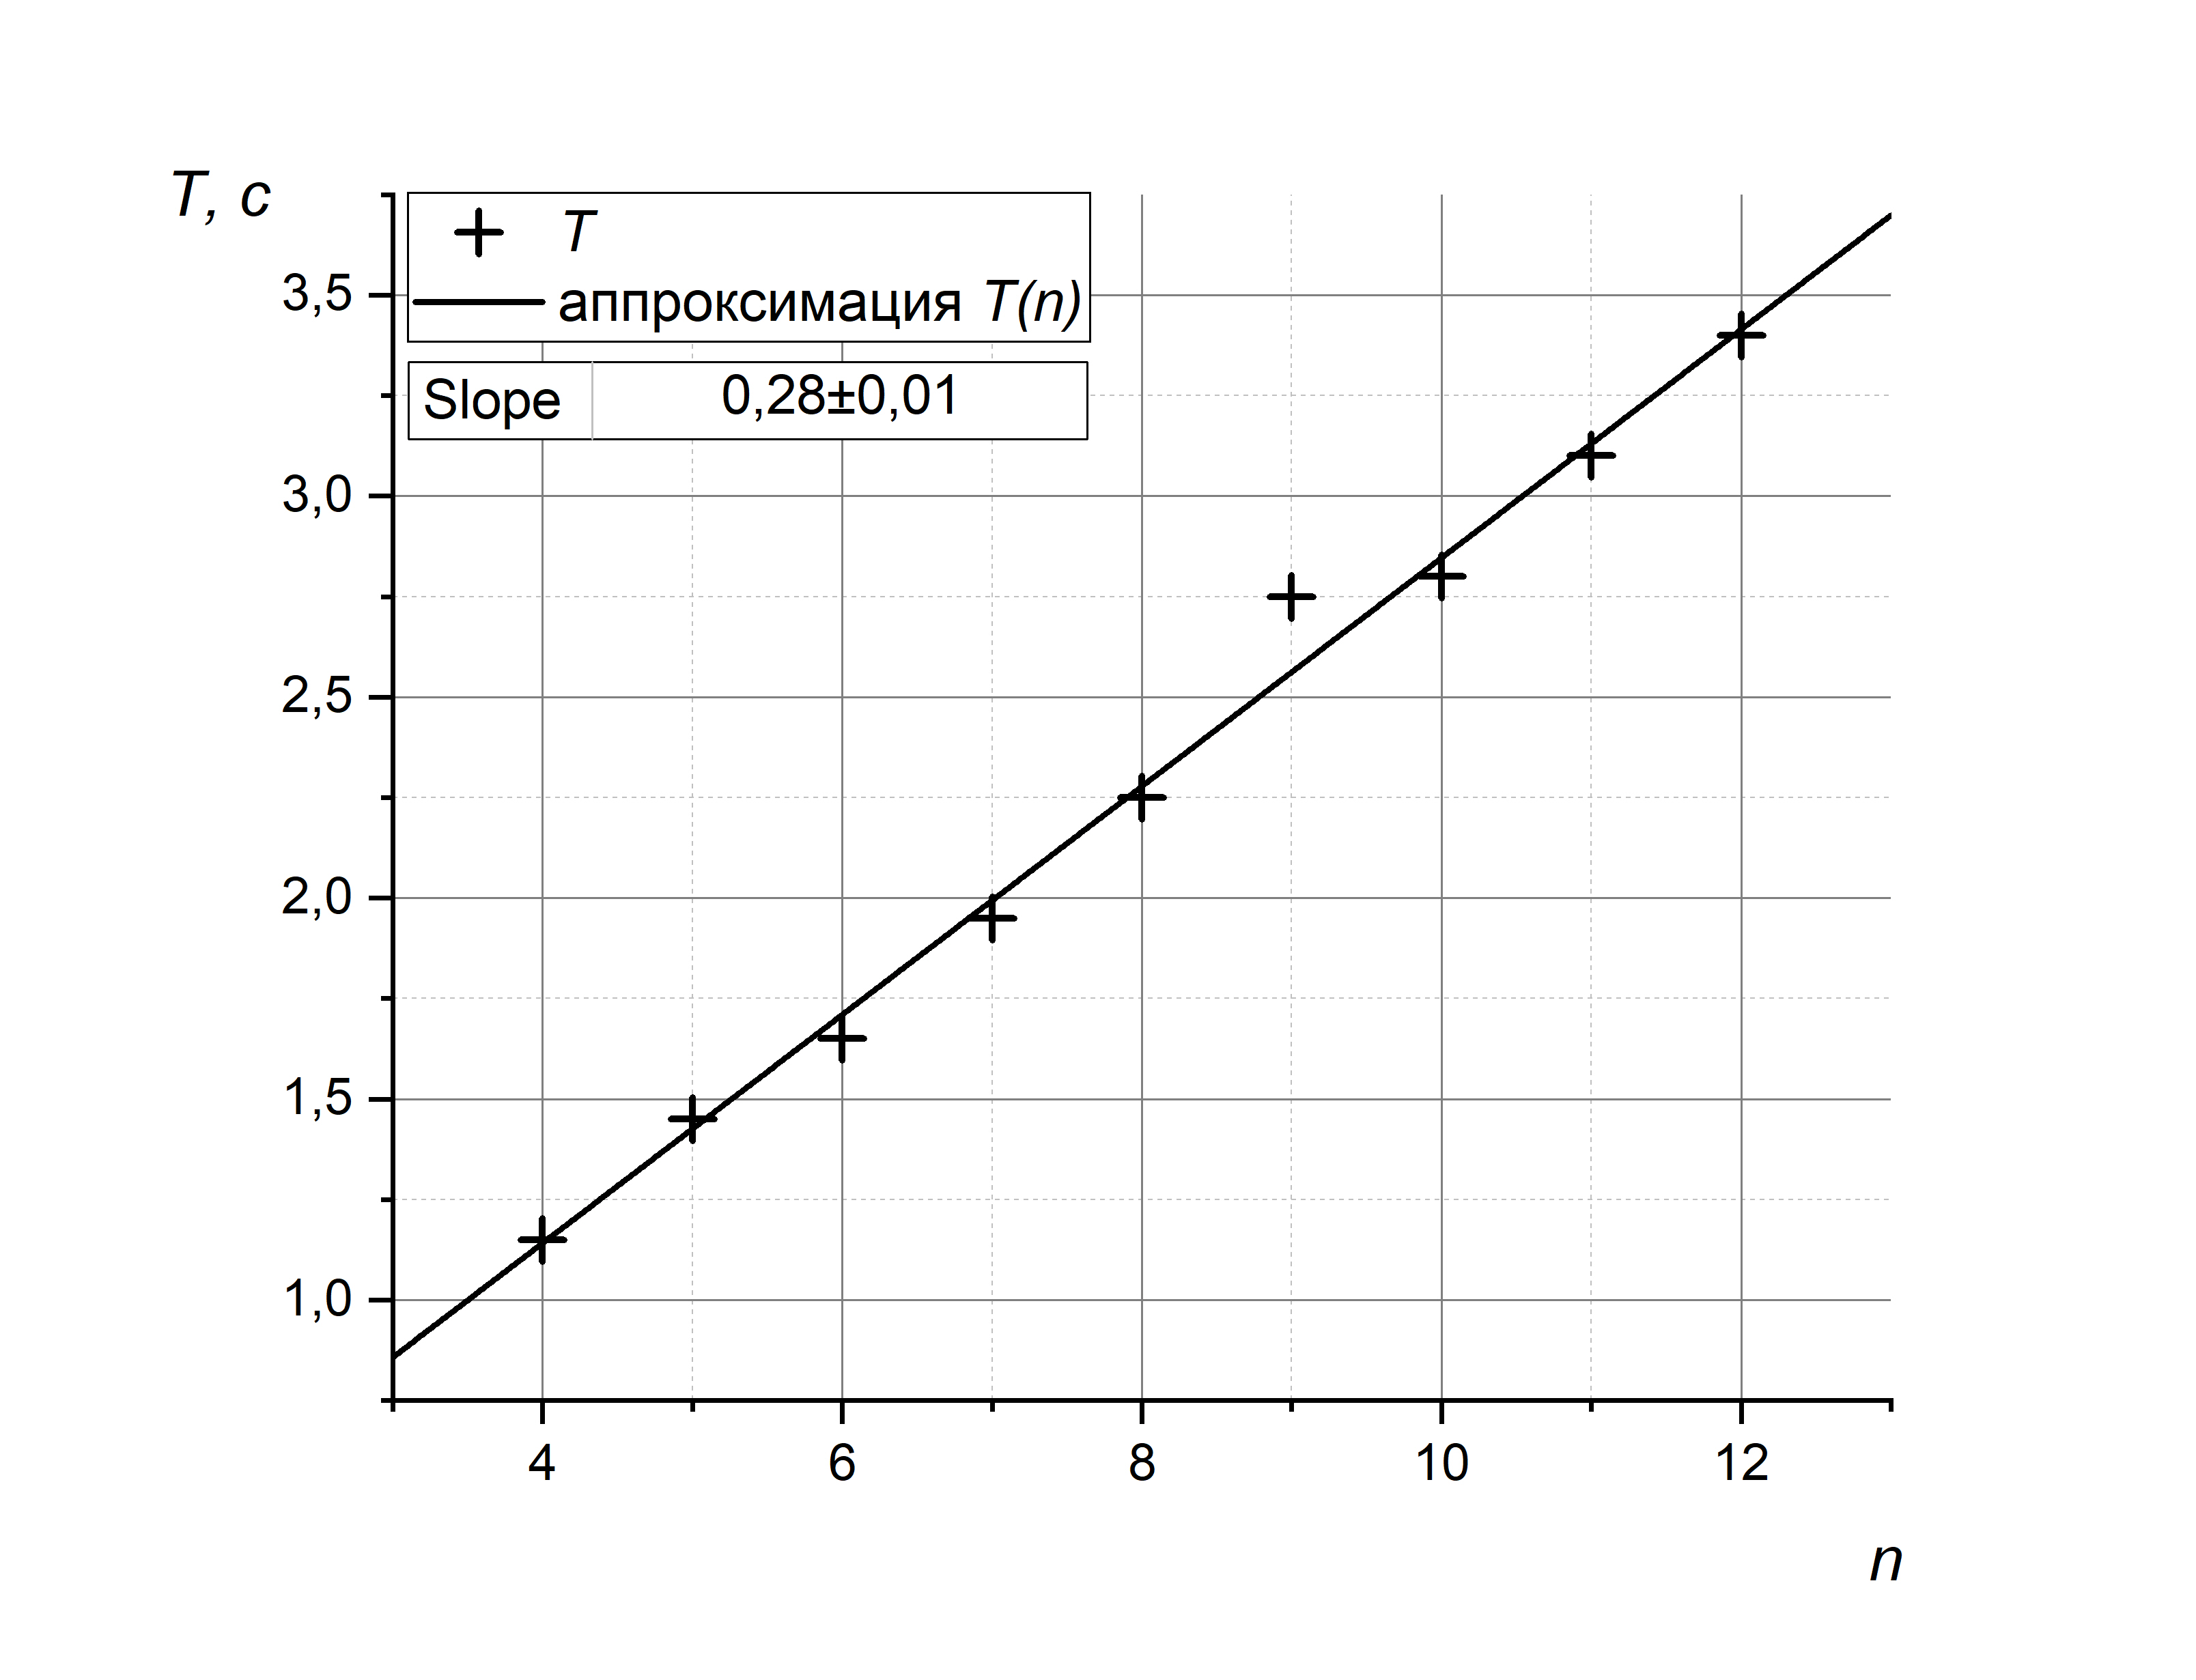
\includegraphics[width = 0.9\textwidth]{2.jpg}\\
\textbf{График 1. } Зависимость $T(n) = k \cdot n$
\end{center}
По значению углового коэффициента $k$ рассчитаем величину горизонтальной составляющей магнитного поля Земли по формуле $(8)$.
\[B_h = (0,144 \pm 0,001) \text{ Гс}\]
\subsection*{Определение вертикальной составляю-щей магнитного поля Земли}
Определяем механический момент сил, действующий со стороны магнитного поля Земли на горизонтально расположенную магнитную "стрелку". Для этого, с помощью одного или нескольких кусочков проволоки, уравновесьте "стрелку" в горизонтальном положении. Сделаем измерения для разных количеств шариков и занесем все в таблицу.
\begin{center}
\begin{tabular}{|c|c|c|c|}
\hline
$n$ & $m$, г & $r$, см & $M$, дин $\cdot$ см \\ \hline
12 & 0,16 & 3 & 470,4 \\ \hline
10 & 0,2 & 2,4 & 470,4 \\ \hline
8 & 0,23 & 1,8 & 405,72 \\ \hline
6 & 0,29 & 1,2 & 341,04 \\ \hline
4 & 0,41 & 0,6 & 241,08 \\ \hline
\end{tabular}\\
\textbf{Таблица 5.} Зависимость момента сил от $n$.
\end{center}
Построим график. 
\begin{center}
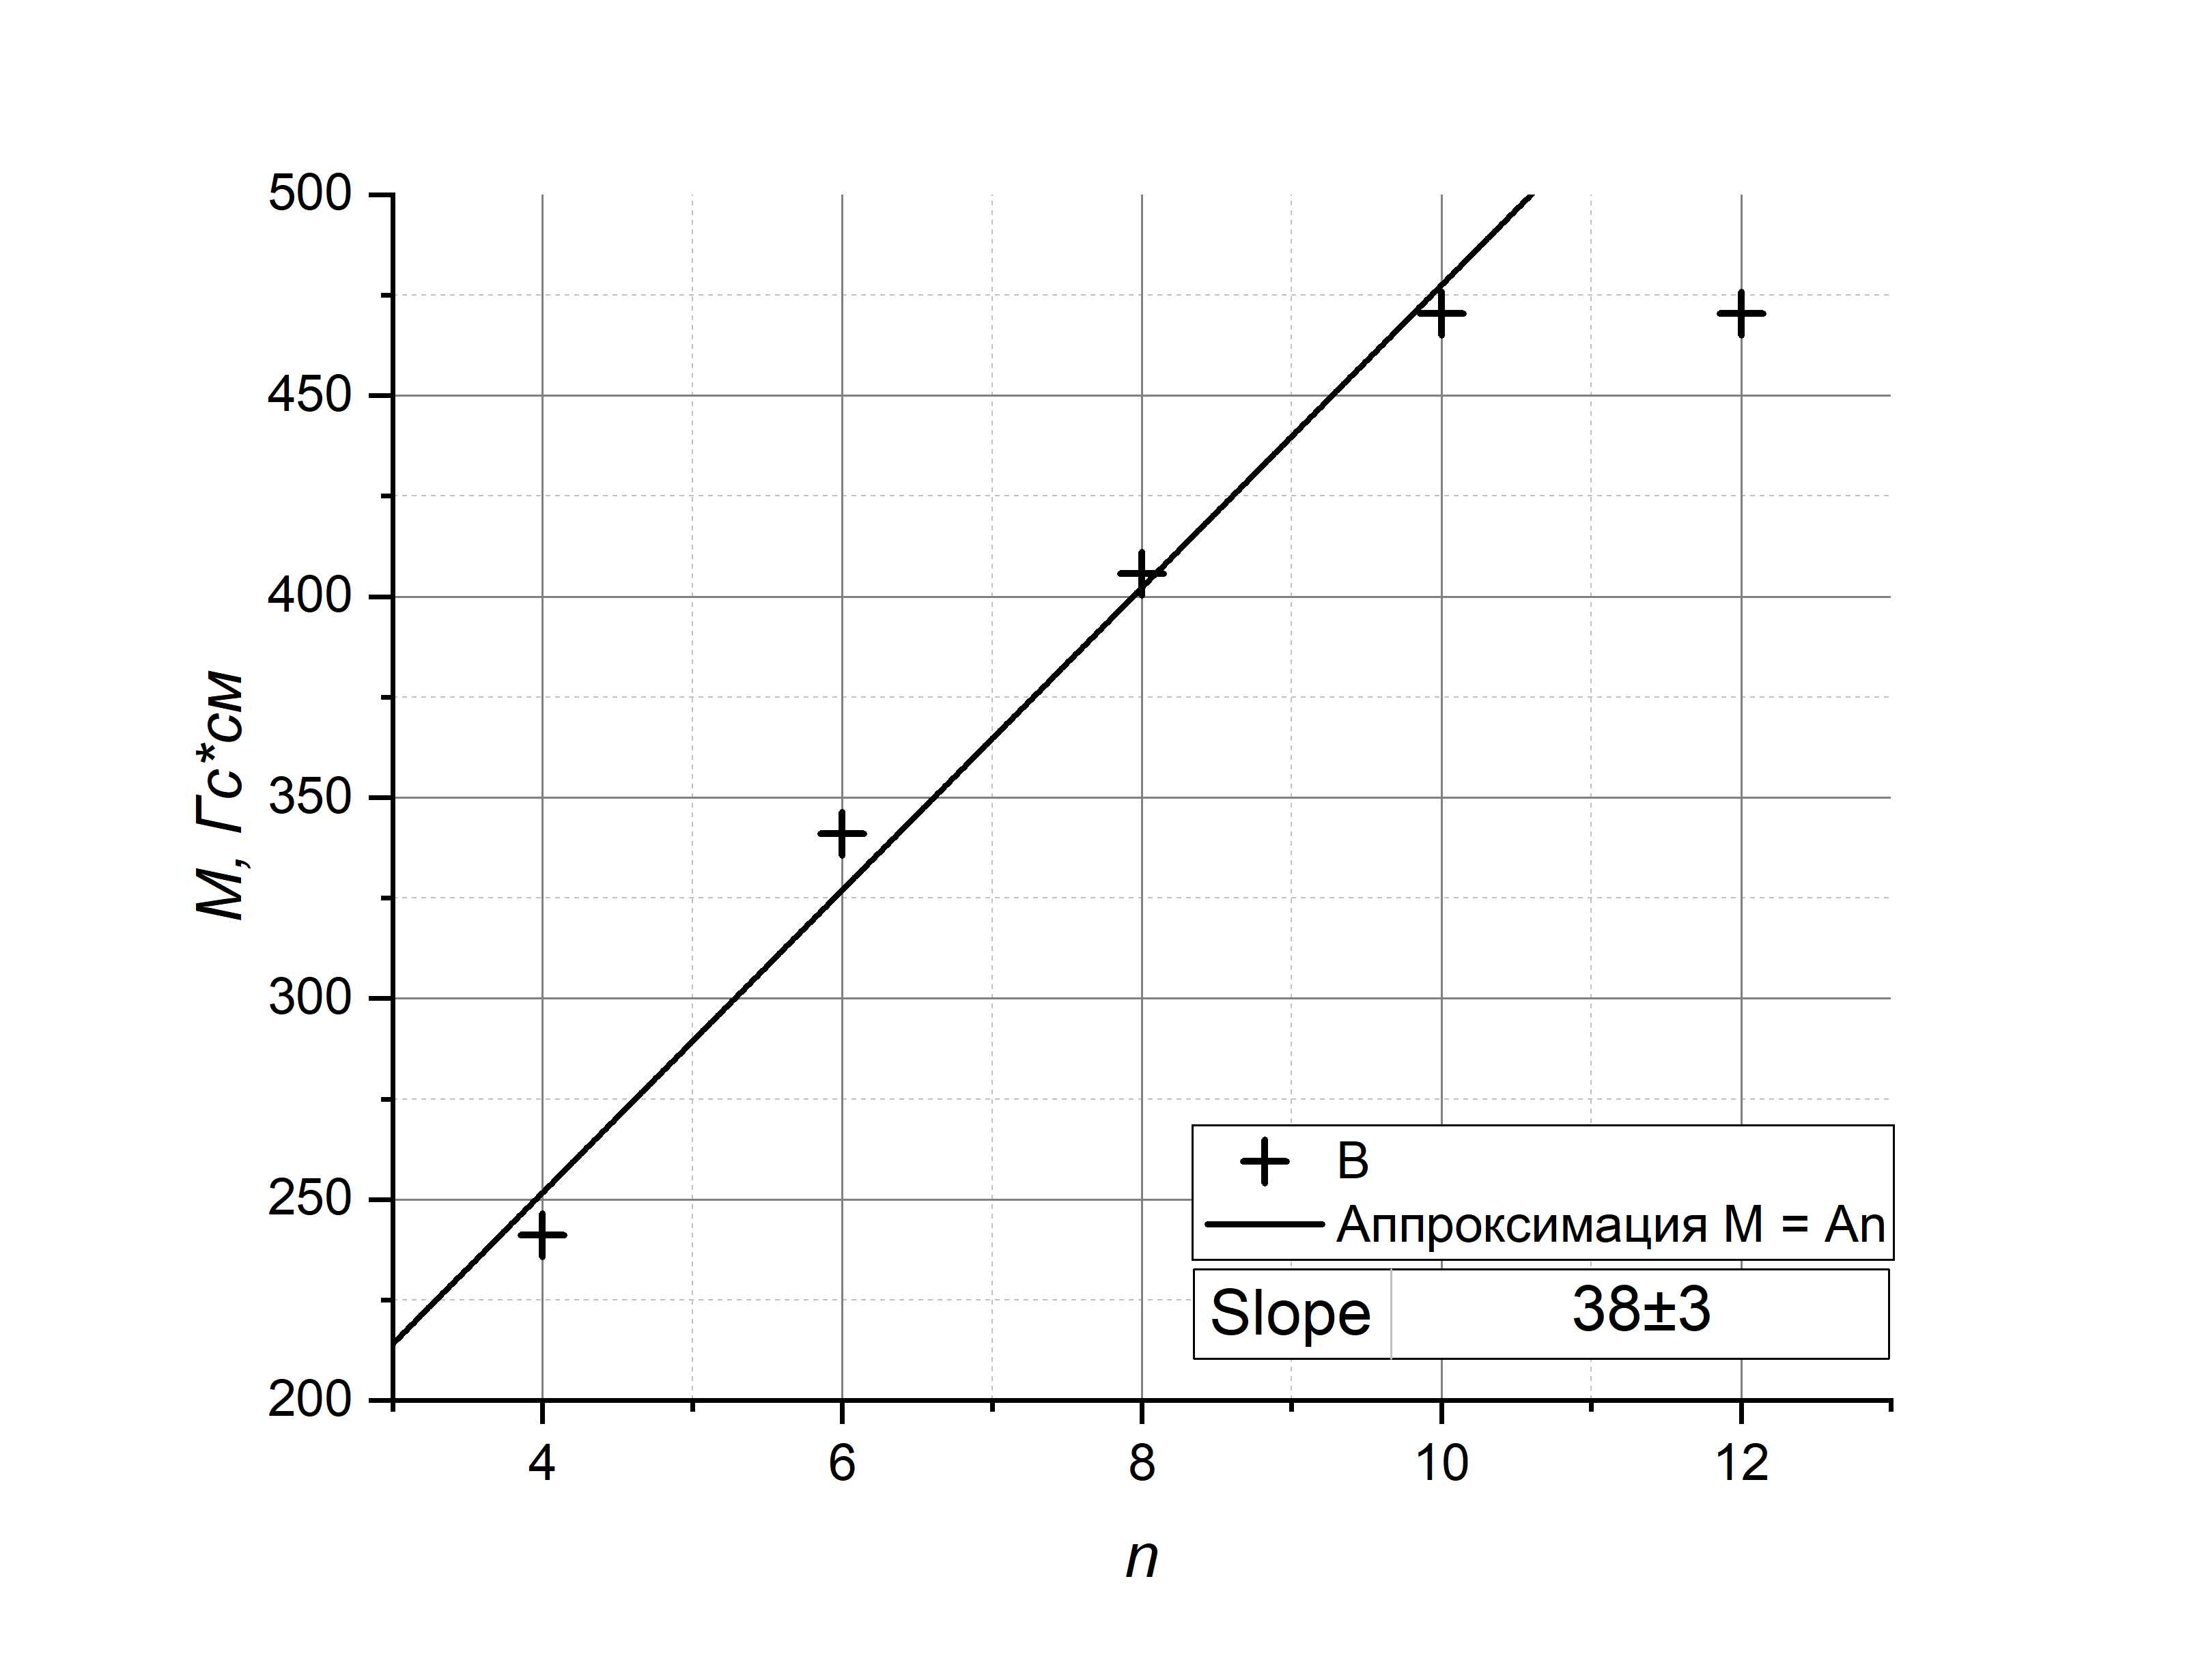
\includegraphics[width = 0.9\textwidth]{3.jpg}\\
\textbf{График 1. } Зависимость $M(n) = A \cdot n$
\end{center}
По формуле $(9)$ определяем $B_v = (0,43 \pm 0,01)$ Гс.

В итоге получаем, что $B = (0,46 \pm 1)$ Гс и $\beta = 72^{\circ}$, что очень близко к современным данным в нашем регионе.
\section*{Используемая литература.}
\begin{enumerate}
\item \textbf{Лабораторный практикум по общей физике:} Учебное пособие. В трех томах. Т. 2. Электричество и магнетизм /Гладун А.Д., Александров Д.А., Берулёва Н.С. и др.; Под ред. А.Д. Гладуна - М.: МФТИ, 2007. - 280 с.
\item \textbf{Дополнительное описание лабораторной работы 1.2.1}: Определение магнитного поля Земли; Под ред. МФТИ, 2015. - 9 с.
\end{enumerate}
\end{document}